\section{结果与讨论}
\label{sec:results}

第一个问题是动作集是否有值得路由的东西。表~\ref{tab:complementarity} 与
图~\ref{fig:headroom} 在逐行层面回答这个问题。总互补
性并不稀缺。在 CodeXGLUE 与 Laya 上，\choice{} 修复了 60 个 \noul{} 错误中
的 14 个，逐行 oracle 达到 0.783 准确率，而更好的固定动作为 0.550，上限为
0.233。同一单元也说明上限为什么是一个糟糕的承诺：\choice{} 破坏了 15 个
正确的 \noul{} 答案，因此训练池上的净计数为 $-1$，净修复区间跨零。其他三个
二元单元的总机会更小（上限 0.067--0.100），净计数在 $-6$ 到 $+1$ 之间。
在四个单元中，训练池从未产生与零可区分的净修复。

留出池没有把总机会转化为稳定的净收益。CodeXGLUE/Laya 单元在
\texttt{selection\_dev} 上提高 20.0 点（$[+1.7,+38.3]$），但同一冻结方向
在 confirm 上只提高 1.7 点（$[-18.3,+20.0]$）。这一差距是选择池效应，而
不是路由效应：dev 正是选择方向的那个池。FinDVer 与 Laya 是检验叙事的例外。
其 confirm 净修复为 $+13.6$ 点 $[+2.0,+24.6]$，固定动作准确率差为 $+0.136$
$[+0.020,+0.246]$。然而相应的 macro-F1 差为 $+0.111$，区间跨零，且更好的
固定动作从 dev 上的 \noul{} 反转为 confirm 上的 \choice{}。因此该单元在
confirm 上含有真实的准确率层面修复信号，但没有 macro-F1 收益，也没有一个
train 选出的策略本会知道去利用的方向。CodeXGLUE 与 Vela 走向相反：冻结方向
是 \choice{} 到 \noul{}，train 净值为 $-6$，confirm 恰好为零。FinDVer 与
Vela 在 confirm 上为负（$-2.3$ 点）。互补性存在于动作集中，但稀疏、依赖
指标且依赖池。

因为 macro-F1 是主指标，我们也计算 dev 与 confirm 上的固定动作差。
\choice{} 减 \noul{} 在 CodeXGLUE/Laya 上为 $+0.074$ $[-0.093,+0.248]$ 与
$-0.127$ $[-0.287,+0.034]$；CodeXGLUE/Vela 为 $+0.003$ $[-0.194,+0.197]$ 与
$+0.078$ $[-0.111,+0.253]$；FinDVer/Laya 为 $-0.072$ $[-0.220,+0.046]$ 与
$+0.111$ $[-0.007,+0.218]$；FinDVer/Vela 为 $-0.106$ $[-0.204,+0.021]$ 与
$-0.106$ $[-0.217,+0.015]$。所有区间都包含零，因此没有固定动作的 macro-F1
差异显著；FinDVer/Laya 在准确率层面的正净修复没有转化为 macro-F1 收益。

\begin{table}[t]
\centering
\footnotesize
\caption{动作互补性，train 选出的方向跨池冻结（每训练单元 $n=60$；FinDVer dev/confirm：59/44）。\emph{上限}
是逐行 oracle 相对 \texttt{search\_train} 上更好固定动作的准确率增益；
\emph{修复/有害}统计替代动作修复或破坏基础决策的行数。净修复是配对差值
（百分点，替代动作减基础动作），dev 与 confirm 上给出 95\% 分组自助法区间。
上限是上界，不是可部署增益。}
\label{tab:complementarity}
\begin{tabular}{@{}llrrrr@{}}
\toprule
任务 / 模型 & 方向 & 上限 & 修复/有害 & dev 净 (95\% CI) & confirm 净 (95\% CI) \\
\midrule
CodeXGLUE / Laya & Noul$\to$Choice & 0.233 & 14/15 & +20.0 [+1.7, +38.3] & +1.7 [-18.3, +20.0] \\
CodeXGLUE / Vela & Choice$\to$Noul & 0.067 & 4/10 & -3.3 [-15.0, +8.3] & +0.0 [-15.0, +15.0] \\
FinDVer / Laya & Noul$\to$Choice & 0.083 & 5/6 & -6.8 [-23.3, +6.0] & +13.6 [+2.0, +24.6] \\
FinDVer / Vela & Choice$\to$Noul & 0.100 & 6/7 & +0.0 [-9.1, +11.5] & -2.3 [-10.3, +5.0] \\
\bottomrule
\end{tabular}
\end{table}


\begin{figure}[t]
\centering
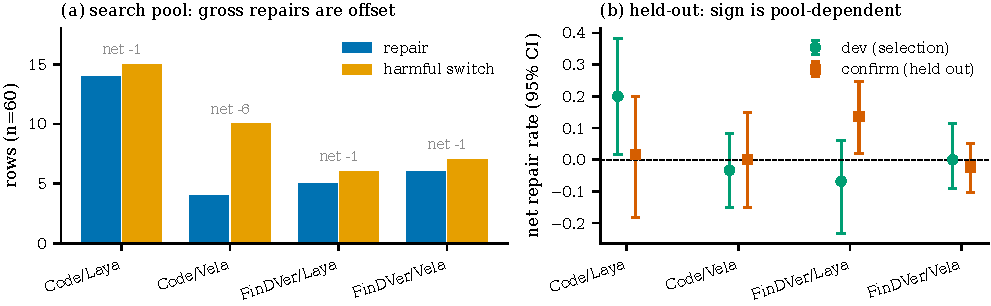
\includegraphics[width=0.92\linewidth]{../acl/figures/fig_headroom.pdf}
\caption{动作互补性。(a) 在训练池上，第二个动作修复错误，但也破坏正确答案；
每对柱上方印有净计数。(b) 同一 train 选出方向应用到 dev 与 confirm：净修复
的符号跨池变化，只有一个 confirm 单元的区间高于零。}
\label{fig:headroom}
\end{figure}

修复出现的位置与数量同样重要。把修复率对 \noul{} 概率分箱作图，
修复集中在中间与高带，约
$p\in[0.4,0.8]$，在最低带接近零。这与置信度级联的假设相反：阈值规则在
模型不确定时切换，而这恰恰是 \choice{} 最不可能修复任何东西的地方，因为
它能修复的行是 \noul{} 自信却错误的地方。这也解释了为什么校准救不了路由：
重校准单调地移动概率质量，但不会把可修复行从分布中部移到低置信度尾部。

第二个问题是 \choice{} 的有符号增量价值能否从第一次调用预测。表~\ref{tab:predictability}
使用 $\Delta_i=\mathbf{1}[\choice_i\text{ 正确}]-
\mathbf{1}[\noul_i\text{ 正确}]\in\{-1,0,+1\}$。所选模型的折外预测与真实
$\Delta$ 的 Spearman 相关为 $-0.02$、$+0.19$、$+0.13$ 和 $-0.17$；每个
分组自助法区间都包含零。有符号 $\Delta$ 的修复 AUROC 为 0.36、0.74、0.46
和 0.40，退化 AUROC 为 0.61、0.33、0.71 和 0.36。dev 选择的阈值（按成本
调整效用选择）给出的 confirm 原始净值为 $0.0$、$0.0$、$0.0$ 和 $-2.3$ 点，
成本调整净值为 $0.0$、$0.0$、$-0.1$ 和 $-2.8$ 点；没有单元为正，
FinDVer/Vela 的成本区间 $[-7.5,-0.1]$ 在负侧排除零。CodeXGLUE/Vela 选择
从不切换（0/60），因此两者都恰为零。始终切换基线为 $+1.7$、$0.0$、
$+13.6$ 和 $-2.3$，因此预测器放弃了 FinDVer/Laya 的全部 $+13.6$ 收益和
CodeXGLUE/Laya 的 $+1.7$ 收益。修复目标预测器达到更高的修复 AUROC
（最高 0.92），但同样在 confirm 上失败：排序修复不等于排序净效用。这里的
修复 AUROC 使用拟合的有符号 $\Delta$ 分数；下面的校准分析使用原始
\noul{} 概率，是另一个量。

\begin{table}[t]
\centering
\footnotesize
\caption{增量效用预测。折外 AUROC 在 \texttt{search\_train} 上使用分组感知
三折交叉验证；冠军模型与阈值在 \texttt{search\_dev} 上选择，冻结后用于
\texttt{confirm}。净效用为（修复 $-$ 退化）$/n$，单位为百分点，括号内为
计数；最后一列每次额外调用减去 $\lambda=0.05$。}
\label{tab:predictability}
\begin{tabular}{@{}lrrlrrr@{}}
\toprule
任务 / 模型 & LogReg 折外 & 树 折外 & 冠军 & dev 净 & confirm 净 & confirm 成本调整 \\
\midrule
CodeXGLUE / Laya & 0.674 & 0.739 & logreg & +20.0 (23/11) & +1.7 (17/16) & -3.3 \\
CodeXGLUE / Vela & 0.716 & 0.646 & logreg & +3.3 (7/5) & -1.7 (9/10) & -6.4 \\
FinDVer / Laya & 0.455 & 0.466 & tree & +1.7 (1/0) & +2.3 (1/0) & +1.5 \\
FinDVer / Vela & 0.919 & 0.794 & logreg & +3.4 (4/2) & -2.3 (0/1) & -2.6 \\
\bottomrule
\end{tabular}
\end{table}


校准是对基于概率的路由失败最自然的解释，因此它作为对照。原始概率在
confirm 上校准很差：ECE 从 0.090 到 0.290，Brier 从 0.218 到 0.287。在
\texttt{search\_train} 上拟合的温度缩放在三个单元降低 ECE（到
0.045--0.169）与 Brier；FinDVer/Vela 的 ECE 与 Brier 都略升。可达到的
band 类别不变，但选出的策略移动：原始概率给出的 confirm 净修复为
$-5.0$、$0.0$、$+2.3$ 与 $-2.3$ 点，温度缩放后为 $-1.7$、$+1.7$、$0.0$
与 $0.0$，与阈值选择噪声一致，而不是新信号。
原始 \noul{} 概率的修复 AUROC 直接说明了这一点：四个单元分别为 0.791、
0.444、0.336 与 0.095；
在后两个单元中，概率把可修复行排到随机水平\emph{之下}。当前答案的校准概率
不是替代动作价值的校准概率。

第三个问题是搜索能否把已有信号转化为可部署策略。表~\ref{tab:search} 总结
了比较。GA 对随机搜索是优化器价值最干净的检验：五个种子、四个任务—模型
单元与三个池，共 60 组配对 macro-F1 比较，没有任何一组的区间排除零。GA 对
固定仅切换有五个显著正单元，全部在 FinDVer/Vela 训练池，效应约为 $+0.12$；
在 dev 与 confirm 上，40 组比较没有一组显著。预注册的部署比较——train 选出
的 GA 对 confirm 上的固定仅切换——在每个种子级单元中都不显著。ES 对随机
搜索在全部 30 组比较中不显著；ES 对固定切换有三个显著训练单元与一个显著
confirm 单元（CodeXGLUE/Laya，种子 17，$+0.176$），这是唯一的 confirm 级
正结果，且未在种子上复现。NSGA-II 部署在五个 dev 单元与一个 confirm 单元
中显著差于固定基线，没有正单元。搜索问题没有任何稳定的留出信号供任何优化器
发现。

\begin{table}[t]
\centering
\small
\caption{预注册协议下的搜索比较。计数为排除零的配对分组自助法 95\% 区间数；
“正”表示演化策略胜过所述基线。GA 与 ES 行在三个池、五个种子上使用
macro-F1；NSGA-II 行在 12 个 dev 与 12 个 confirm 单元上使用准确率。}
\label{tab:search}
\begin{tabular}{@{}lrrl@{}}
\toprule
比较 & 正 & 负 & 解读 \\
\midrule
GA 对随机 & 0 & 0 & 无优势 (60) \\
GA 对固定 & 5 & 0 & 仅训练池 (60) \\
ES 对随机 & 0 & 0 & 无优势 (30) \\
ES 对固定 & 4 & 0 & 一个 confirm (30) \\
NSGA-II 对固定 & 0 & 6 & 5 dev, 1 confirm \\
\bottomrule
\end{tabular}
\end{table}


轨迹诊断解释了为什么更多搜索没有帮助。在 21 次记录的 GA/ES 运行中，有 15
次的最优适应度在第 0 代之后不再提高。中性变异率为 0.68--0.73，因此大多数
变异产生的候选训练分数完全相同。两个 CodeXGLUE 单元的 train--dev 秩相关为
$-0.56$ 与 $-0.51$，意味着在 train 上看起来更好的候选在 dev 上往往更差；
FinDVer 单元为 $+0.44$ 与 $+0.99$。把 CodeXGLUE/Vela 的预算从 24 提高到
48 并没有缩小差距：GA 在 48 的上限下只评估了 22、17 与 23 个唯一基因组，
而随机搜索用满了 48 个。搜索不只是调参不足，而是信息不足。

锁定测试是最后检查。每个单元使用 60 条官方 test 行，模板与 GA 基因组在
任何 test 调用前冻结；GA 对固定切换的 macro-F1 差为 $+0.008$
$[-0.148,+0.163]$（CodeXGLUE/Laya）、$0.000$ $[0.000,0.000]$
（CodeXGLUE/Vela）、$0.000$ $[-0.046,+0.045]$（FinDVer/Laya）与 $+0.243$
$[+0.138,+0.318]$（FinDVer/Vela）。最后一个增益来自更差的固定动作：固定
切换 macro-F1 为 0.413，固定 \noul{} 为 0.677，而 GA 基本停留在 \noul{}
（1.00--1.05 次调用/行），并未胜过 \noul{}（seed 17 为 $-0.021$
$[-0.081,0.000]$；seed 23/41 为 0）。没有任何 GA 基因组在任何单元上胜过
更好的固定动作。

边界检查问这些结论是否是某个池或任务的产物。迁移一致地没有帮助：32 个
源—目标乘划分单元中六个显著，且全部为负（两个对角线，四个非对角线）。
故障图确认 15 个合格单元中的 13 个在 dev、10 个在 confirm；稳定的高严重度
区域是 ProcessBench 的中置信度带，两个模型在同一批行上一起失败。

表~\ref{tab:processbench} 报告同一池上的选择性预测基线。全覆盖时选择性
准确率为 Laya 0.133、Vela 0.083；50\% 目标覆盖为 0.100/0.069，25\% 为
0.105/0.143；AURC 为 0.894/0.883。置信度不足以让弃权买到准确率。

\begin{table}[t]
\centering
\small
\caption{ProcessBench 在 confirm 上的选择性预测。各列为全覆盖、50\% 目标覆盖与
25\% 目标覆盖下的选择性准确率；括号内为实际 confirm 覆盖率。阈值在
\texttt{selection\_dev} 上选择并冻结。AURC 为风险—覆盖曲线下面积（越低越好）。}
\label{tab:processbench}
\begin{tabular}{@{}lrrrr@{}}
\toprule
模型 & 全覆盖 & 50\% 目标 & 25\% 目标 & AURC \\
\midrule
Laya & 0.133 (1.00) & 0.100 (0.50) & 0.105 (0.32) & 0.894 \\
Vela & 0.083 (1.00) & 0.069 (0.48) & 0.143 (0.23) & 0.883 \\
\bottomrule
\end{tabular}
\end{table}


综合来看，三个问题描述了一个在优化器被要求解决之前就已经失败的路由问题：
RQ1 发现总互补性但没有稳定的净互补性，RQ2 发现排序信号但没有可靠的策略
价值，RQ3 发现没有留出优势，因为地形平坦，而且训练排序在关键处不能预测
dev 排序。校准改进的是另一个量：模型可以为它回答的问题报告更好的概率，
却仍然无法说明另一个问题是否会被回答得更好。

实践含义是工作顺序的改变。在构建路由器之前，先测量动作集在留出组上是否
有净互补性，以及候选特征能否把可修复行排到随机水平之上。如果任一检查失败，
更强的优化器不会有用；如果两者都通过，就可以在匹配预算下运行优化器比较，
并使用预注册的 confirm 比较。
